\chapter{GuiltyTargets: prioritization of novel therapeutic targets with deep network tepresentation learning}
\label{ch:guiltytargets}

\section*{Preface}

The choice of a target protein whose modulation may cause a therapeutic effect in a target disease is essential for success in drug discovery.
Unfortunately, the majority of clinical trials fail due to low efficacy, often attributed to a poor choice of target protein.
Computational target prioritization approaches aim to support target selection by ranking candidate targets in the context of a given disease.
The following publication presents a novel target prioritization approach, GuiltyTargets, which relies on network representation learning of protein-protein interaction networks annotated with disease-specific differential gene expression.
These techniques are not only useful in investigation of new diseases, but also in the attribution of previously studied drugs to new indications when their targets can be shown to be relevant in new therapeutic indications.

\vspace*{\fill}

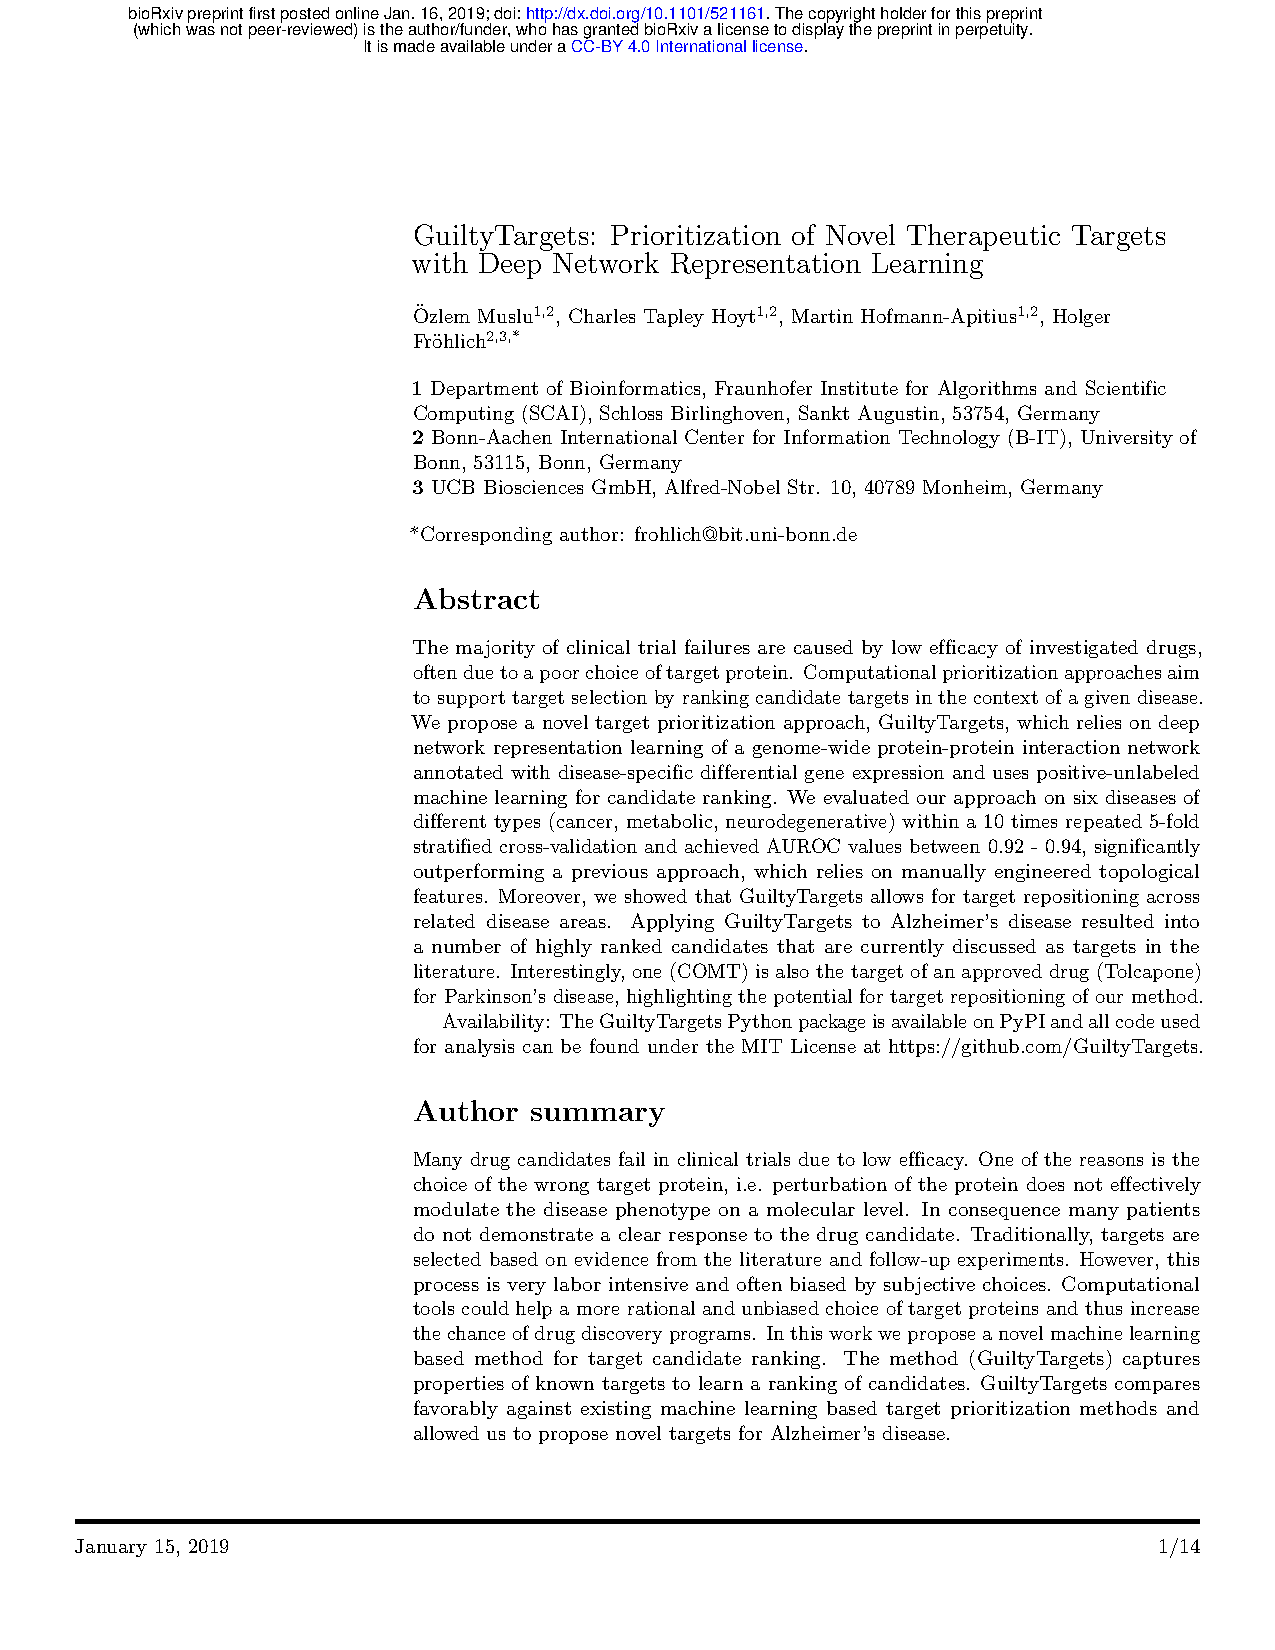
\includepdf[pages={-}]{articles/guiltytargets.pdf}

\section*{Postface}

The exchange of engineered topological features for learned features increased the performance in target prioritization across nearly all combinations of protein-protein interaction databases (i.e., HIPPIE and STRING), disease-target association databases (i.e., Therapeutic Target Database and OpenTargets), and other hyperparameters used in the workflow from Emig \textit{et al.}~\cite{Emig2013}.
While initial work used the same protein-protein interaction networks and disease-specific differential gene expression profiles, it can be extended to accomodate the rich knowledge encoded in \ac{BEL} networks generated by manual, semi-automated, and automated approaches described elsewhere in this thesis.
Future work could also easily incorporate the networks arising from Bio2BEL packages presented in Chapter~\ref{ch:bio2bel}.